\documentclass[aspectratio=169,10pt]{beamer}
\usepackage{../common/beamer_theme_bio}

\title{\textbf{Biostatistiques Appliquées \& Modélisation du Vivant}}
\subtitle{Chapitre I : Analyse de Variance (ANOVA) à Deux Facteurs Croisés \& Interactions}
\author{\textbf{Dr. Sarra BENMOUMOU (Ph.D.)}}
\institute{
  Faculté des Sciences --- Département de Biologie\\
  Master 2 : Biochimie Appliquée\\
  \textbf{Université M'Hamed Bougara de Boumerdès (UMBB)}
}

% Intercalaire automatique de transition entre sections (Plein écran sans débordement)
\AtBeginSection[]{
  \begin{frame}[plain]
    \vspace{1mm}
    \begin{tcolorbox}[colback=BioNavy,coltext=white,boxrule=0pt,arc=2mm,left=6pt,right=6pt,top=2pt,bottom=2pt]
      \centering\bfseries\small Progression Pédagogique du Cours
    \end{tcolorbox}
    \vspace{0.5mm}
    {\scriptsize\tableofcontents[currentsection, hideothersubsections]}
  \end{frame}
}

\begin{document}

% --- Page de Titre ---
\begin{frame}[plain]
  \titlepage
\end{frame}

% --- Sommaire Général ---
\begin{frame}{Plan Détaillé du Chapitre I}
  \tableofcontents
\end{frame}

% ========================================================
\section{Motivation \& Démarche des Plans Factoriels Croisés}
% ========================================================

\begin{frame}{Pourquoi Passer à Deux Facteurs Simultanés ?}
  \begin{columns}[onlytextwidth, T]
    \begin{column}{0.48\linewidth}
      \begin{warnbox}{Le Piège du « Un Facteur à la Fois » (OFAT)}
        \small
        L'approche historique testait séparément la molécule antioxydante puis le génotype.\\
        \textbf{Limites majeures :}
        \begin{itemize}
          \item Ignore l'effet combiné (\textbf{synergie} ou \textbf{antagonisme}).
          \item Multiplie les animaux sacrifiés (contraire aux 3R).
          \item Gonfle le risque d'erreur globale $\alpha$.
        \end{itemize}
      \end{warnbox}
    \end{column}
    \begin{column}{0.48\linewidth}
      \begin{conceptbox}{La Richesse du Plan Factoriel}
        \small
        En recherche biomédicale, les mécanismes sont intriqués :
        \begin{itemize}
          \item Efficacité dépendant du \textbf{sexe} ou du \textbf{génotype}.
          \item Activité enzymatique liant \textbf{pH} et \textbf{température}.
          \item Survie cellulaire fonction de la \textbf{dose} et du \textbf{temps}.
        \end{itemize}
        $\implies$ L'ANOVA à deux facteurs teste \textbf{simultanément} les variables et leur synergie dans un plan unique optimisé.
      \end{conceptbox}
    \end{column}
  \end{columns}
\end{frame}

\begin{frame}{Structure d'un Plan Factoriel Croisé Équilibré ($I \times J$)}
  \begin{columns}[onlytextwidth, T]
    \begin{column}{0.48\linewidth}
      \begin{conceptbox}{Définition du Plan Croisé Équilibré}
        \small
        Dans un \textbf{plan factoriel croisé ($A \times B$)} :
        \begin{itemize}
          \item Facteur A : $I$ modalités ; Facteur B : $J$ modalités.
          \item \textbf{Croisement complet :} $I \times J$ combinaisons testées.
          \item \textbf{Plan équilibré :} $K$ réplicats identiques par lot.
          \item \textbf{Effectif total :} $N = I \cdot J \cdot K$ individus.
        \end{itemize}
      \end{conceptbox}
    \end{column}
    \begin{column}{0.48\linewidth}
      \begin{biobox}{Exemple Concret au Laboratoire}
        \small
        Étude préclinique d'un hépatoprotecteur :
        \begin{itemize}
          \item \textbf{Facteur A (Dose) :} $I = 3$ (Témoin, 50, 100 mg/kg).
          \item \textbf{Facteur B (Génotype) :} $J = 2$ (WT vs $db/db$).
          \item $K = 5$ souris par condition $\implies 6$ lots.
          \item \textbf{Effectif total :} $N = 3 \times 2 \times 5 = 30$ souris.
        \end{itemize}
      \end{biobox}
    \end{column}
  \end{columns}
\end{frame}

\begin{frame}{Notion 1 : L'Effet Principal du Facteur A}
  \begin{columns}[onlytextwidth, T]
    \begin{column}{0.48\linewidth}
      \begin{conceptbox}{Définition Statistique}
        \small
        L'\textbf{Effet Principal} de A mesure l'impact moyen de A en moyennant sur toutes les modalités de B :
        \begin{equation*}
          \alpha_i = \bar{Y}_{i\cdot\cdot} - \bar{Y}_{\dots} \quad \left(\sum_{i=1}^I \alpha_i = 0\right)
        \end{equation*}
        \textbf{Hypothèse nulle testée :}
        \begin{equation*}
          H_0^{(A)} : \alpha_1 = \dots = \alpha_I = 0
        \end{equation*}
      \end{conceptbox}
    \end{column}
    \begin{column}{0.48\linewidth}
      \begin{biobox}{Interprétation Biologique}
        \small
        \textbf{Question posée :} \textit{« Globalement, le traitement modifie-t-il la peroxydation lipidique, quel que soit le statut génétique ? »}
        \begin{itemize}
          \item Si $H_0^{(A)}$ est vraie : aucun effet moyen du traitement.
          \item Si $H_0^{(A)}$ est rejetée ($p \le 0.05$) : au moins une dose diffère significativement des autres.
        \end{itemize}
      \end{biobox}
    \end{column}
  \end{columns}
\end{frame}

\begin{frame}{Notion 2 : L'Effet Principal du Facteur B}
  \begin{columns}[onlytextwidth, T]
    \begin{column}{0.48\linewidth}
      \begin{conceptbox}{Définition Statistique}
        \small
        L'\textbf{Effet Principal} de B quantifie la déviation moyenne propre au facteur B :
        \begin{equation*}
          \beta_j = \bar{Y}_{\cdot j\cdot} - \bar{Y}_{\dots} \quad \left(\sum_{j=1}^J \beta_j = 0\right)
        \end{equation*}
        \textbf{Hypothèse nulle testée :}
        \begin{equation*}
          H_0^{(B)} : \beta_1 = \dots = \beta_J = 0
        \end{equation*}
      \end{conceptbox}
    \end{column}
    \begin{column}{0.48\linewidth}
      \begin{biobox}{Interprétation Biologique}
        \small
        \textbf{Question posée :} \textit{« Indépendamment du traitement, les souris diabétiques ont-elles un stress oxydatif basal différent des souris saines ? »}
        \begin{itemize}
          \item Si $H_0^{(B)}$ est vraie : la mutation n'altère pas le niveau moyen du biomarqueur.
          \item Si $H_0^{(B)}$ est rejetée ($p \le 0.05$) : le génotype crée une différence basale significative.
        \end{itemize}
      \end{biobox}
    \end{column}
  \end{columns}
\end{frame}

\begin{frame}{Notion 3 : La Notion Clé d'Interaction Biologique ($A \times B$)}
  \begin{columns}[onlytextwidth, T]
    \begin{column}{0.48\linewidth}
      \begin{conceptbox}{Définition \& Formule}
        \small
        Il existe une \textbf{interaction} lorsque l'effet du facteur A \textbf{dépend de la modalité de B} :
        \begin{equation*}
          (\alpha\beta)_{ij} = \bar{Y}_{ij\cdot} - (\bar{Y}_{\dots} + \alpha_i + \beta_j)
        \end{equation*}
        $(\alpha\beta)_{ij}$ quantifie l'écart non expliqué par la simple addition des effets simples.
        \begin{equation*}
          H_0^{(AB)} : \text{Tous les } (\alpha\beta)_{ij} = 0
        \end{equation*}
      \end{conceptbox}
    \end{column}
    \begin{column}{0.48\linewidth}
      \begin{biobox}{Exemple en Pharmacologie}
        \small
        \begin{itemize}
          \item Un extrait polyphénolique réduit le MDA de $58\%$ chez les diabétiques ($db/db$).
          \item Mais il n'a aucun effet mesurable ($0\%$) chez les témoins sains (WT).
          \item $\implies$ L'efficacité thérapeutique \textbf{interagit} avec l'état pathologique.
          \item La simple addition $A + B$ échoue à prédire la réponse !
        \end{itemize}
      \end{biobox}
    \end{column}
  \end{columns}
\end{frame}

\begin{frame}{Notion 4 : Synergie vs. Antagonisme Biologique}
  \begin{columns}[onlytextwidth, T]
    \begin{column}{0.48\linewidth}
      \begin{biobox}{1. La Synergie (Interaction Positive)}
        \small
        L'effet combiné est \textbf{supérieur} à la somme des effets isolés :
        \begin{equation*}
          \text{Effet}(A + B) > \text{Effet}(A) + \text{Effet}(B)
        \end{equation*}
        \textbf{Exemple biomédical :}
        \begin{itemize}
          \item $\beta$-lactamine seule : lyse de $20\%$.
          \item Inhibiteur d'enzymes seul : lyse $0\%$.
          \item Association des deux : lyse de $95\%$ !
        \end{itemize}
      \end{biobox}
    \end{column}
    \begin{column}{0.48\linewidth}
      \begin{warnbox}{2. L'Antagonisme (Interaction Négative)}
        \small
        La présence d'un facteur \textbf{inhibe} l'action de l'autre facteur :
        \begin{equation*}
          \text{Effet}(A + B) < \text{Effet}(A) + \text{Effet}(B)
        \end{equation*}
        \textbf{Exemple biochimique :}
        \begin{itemize}
          \item Une molécule activatrice allostérique perd son action stimulatrice si un inhibiteur compétitif bloque le site actif.
        \end{itemize}
      \end{warnbox}
    \end{column}
  \end{columns}
\end{frame}

\begin{frame}{Notion 5 : Lecture Graphique des Profils d'Interaction}
  \begin{center}
    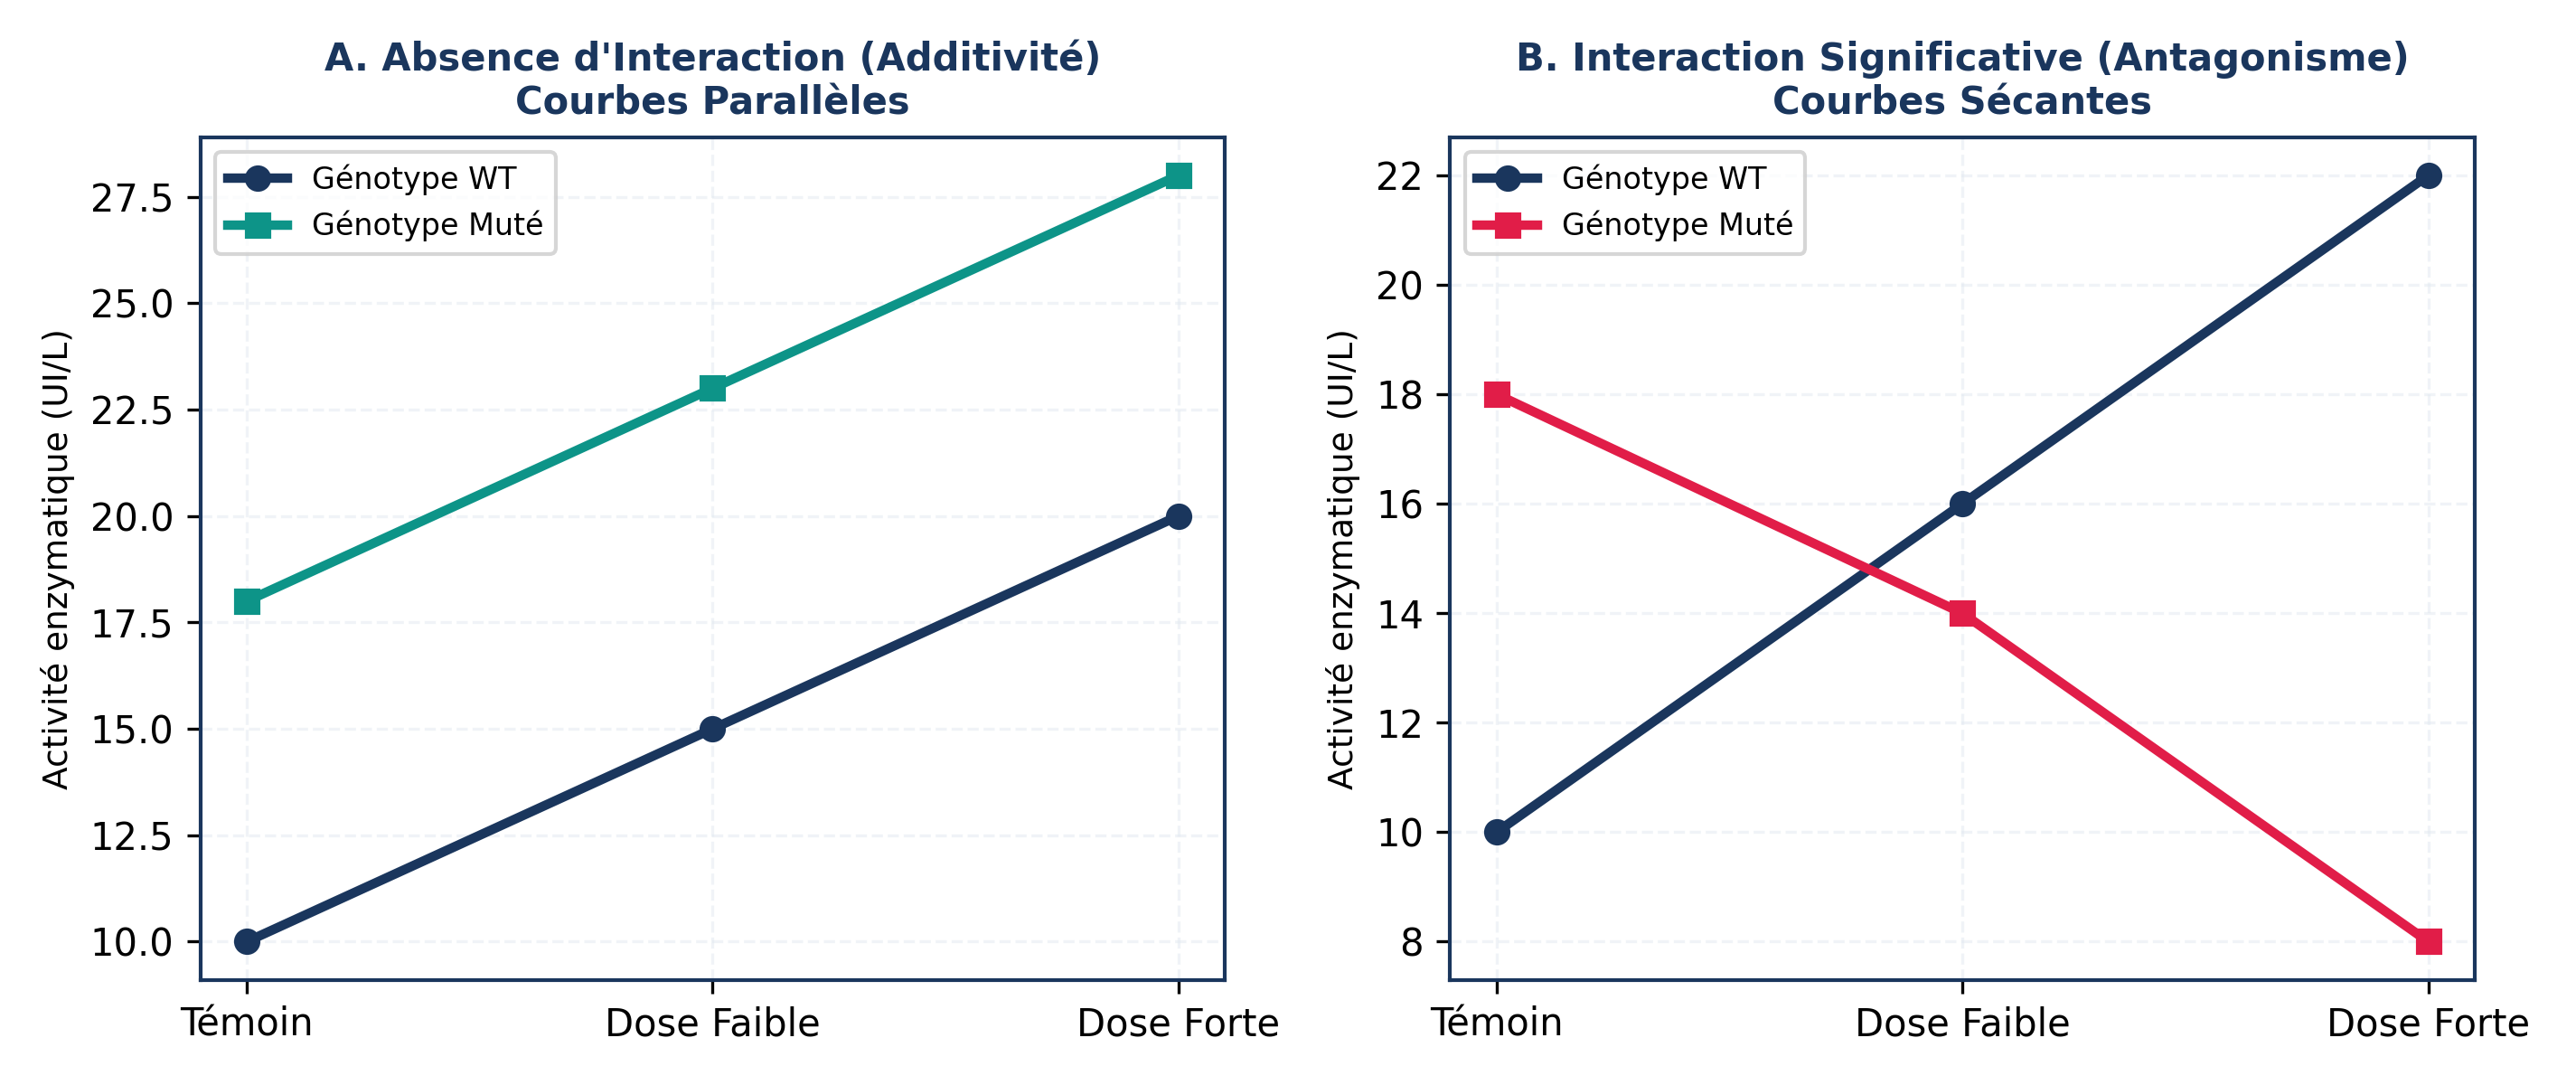
\includegraphics[width=0.62\linewidth, height=3.2cm, keepaspectratio]{../figures/fig01_interaction_profiles.png}
  \end{center}
  \vspace{-2mm}
  \begin{columns}[onlytextwidth, T]
    \begin{column}{0.48\linewidth}
      \textbf{\small\color{BioNavy}Profils Parallèles $\implies$ Additivité Pure}
      \begin{itemize}\small
        \item L'effet de la dose est identique quel que soit le génotype.
        \item Absence formelle d'interaction ($p > 0.05$).
      \end{itemize}
    \end{column}
    \begin{column}{0.48\linewidth}
      \textbf{\small\color{BioRed}Profils Croisés $\implies$ Interaction Forte}
      \begin{itemize}\small
        \item La réponse à la dose diffère selon le génotype.
        \item Interaction hautement significative ($p \le 0.05$).
      \end{itemize}
    \end{column}
  \end{columns}
\end{frame}

\begin{frame}{Notion 6 : Typologie des Modèles (Fixe, Aléatoire, Mixte)}
  \begin{columns}[onlytextwidth, T]
    \begin{column}{0.32\linewidth}
      \begin{conceptbox}{Modèle I : Effets Fixes}
        \begin{itemize}
          \item L'expérimentateur choisit délibérément les modalités (ex: Doses $0, 50, 100\,\text{mg/kg}$).
          \item Les conclusions s'appliquent \textbf{exclusivement} à ces niveaux précis.
          \item \textbf{C'est le cas standard en biochimie.}
        \end{itemize}
      \end{conceptbox}
    \end{column}
    \begin{column}{0.34\linewidth}
      \begin{conceptbox}{Modèle II : Effets Aléatoires}
        \begin{itemize}
          \item Les modalités sont un tirage au sort parmi une infinité (ex: 4 lots de sérum bovin tirés d'un cheptel).
          \item Objectif : Estimer les composantes de variance.
        \end{itemize}
      \end{conceptbox}
    \end{column}
    \begin{column}{0.32\linewidth}
      \begin{conceptbox}{Modèle III : Modèle Mixte}
        \begin{itemize}
          \item Un facteur fixe (ex: Traitement) croisé avec un facteur aléatoire (ex: Opérateur ou Hôpital).
          \item Le dénominateur des tests $F$ change !
        \end{itemize}
      \end{conceptbox}
    \end{column}
  \end{columns}
\end{frame}

% ========================================================
\section{Modélisation Mathématique \& Équations du Modèle}
% ========================================================

\begin{frame}{Notion 7 : L'Équation Linéaire Fondamentale de l'ANOVA Croisée}
  \begin{conceptbox}{Formulation Mathématique Complète}
    Chaque mesure individuelle $Y_{ijk}$ (réplicat biologique $k$ recevant le niveau $i$ de A et le niveau $j$ de B) est décomposée par :
    \begin{equation*}
      Y_{ijk} = \mu + \alpha_i + \beta_j + (\alpha\beta)_{ij} + \varepsilon_{ijk}
    \end{equation*}
    Avec $i = 1, \dots, I$ ; $j = 1, \dots, J$ ; $k = 1, \dots, K$.
  \end{conceptbox}

  \begin{columns}[onlytextwidth, T]
    \begin{column}{0.48\linewidth}
      \textbf{\color{BioNavy}Partie Déterministe (Structurelle) :}
      \begin{itemize}
        \item $\mu$ : Grande moyenne biologique de référence.
        \item $\alpha_i$ : Effet spécifique du traitement $i$.
        \item $\beta_j$ : Effet spécifique du génotype $j$.
        \item $(\alpha\beta)_{ij}$ : Interaction spécifique entre $i$ et $j$.
      \end{itemize}
    \end{column}
    \begin{column}{0.48\linewidth}
      \textbf{\color{BioTeal}Partie Aléatoire (Stochastique) :}
      \begin{itemize}
        \item $\varepsilon_{ijk}$ : Erreur résiduelle biologique.
        \item Capture les micro-variations propres à chaque animal individuel.
        \item \textbf{Postulat fondamental :} $\varepsilon_{ijk} \overset{\text{iid}}{\sim} \mathcal{N}(0, \sigma^2)$.
      \end{itemize}
    \end{column}
  \end{columns}
\end{frame}

\begin{frame}{Notion 8 : Contraintes d'Identifiabilité (Pourquoi Somme = 0 ?)}
  \begin{columns}[onlytextwidth, T]
    \begin{column}{0.48\linewidth}
      \begin{conceptbox}{Le Problème Mathématique}
        Sans contrainte, l'équation linéaire possède une infinité de solutions. Pour fixer des estimateurs uniques, on impose les \textbf{contraintes de centrage} :
        \begin{align*}
          \sum_{i=1}^I \alpha_i &= 0, \quad \sum_{j=1}^J \beta_j = 0 \\
          \sum_{i=1}^I (\alpha\beta)_{ij} &= 0 \; (\forall j), \quad \sum_{j=1}^J (\alpha\beta)_{ij} = 0 \; (\forall i)
        \end{align*}
      \end{conceptbox}
    \end{column}
    \begin{column}{0.48\linewidth}
      \begin{biobox}{Interprétation Biologique Simple}
        \begin{itemize}
          \item Les paramètres $\alpha_i$ et $\beta_j$ sont des \textbf{écarts relatifs à la moyenne générale}.
          \item Si un traitement augmente la réponse de $+4\,\mu\text{mol/g}$, les autres doivent compenser pour que la somme soit nulle.
          \item Les $(\alpha\beta)_{ij}$ mesurent les déviations par rapport au plan additif.
        \end{itemize}
      \end{biobox}
    \end{column}
  \end{columns}
\end{frame}

\begin{frame}{Notion 9 : L'Erreur Résiduelle Biologique $\varepsilon_{ijk}$ \& le Bruit de Fond}
  \begin{columns}[onlytextwidth, T]
    \begin{column}{0.48\linewidth}
      \begin{conceptbox}{Nature Mathématique du Résidu}
        Distance entre la valeur mesurée sur un animal $Y_{ijk}$ et la moyenne théorique de son groupe $\mu_{ij}$ :
        \begin{align*}
          \varepsilon_{ijk} &= Y_{ijk} - \mu_{ij} \\
          &= Y_{ijk} - (\mu + \alpha_i + \beta_j + (\alpha\beta)_{ij})
        \end{align*}
        \begin{itemize}
          \item Centré sur zéro : $\mathbb{E}(\varepsilon_{ijk}) = 0$.
          \item Variance constante : $\mathrm{Var}(\varepsilon_{ijk}) = \sigma^2$.
        \end{itemize}
      \end{conceptbox}
    \end{column}
    \begin{column}{0.48\linewidth}
      \begin{biobox}{Sens Expérimental à la Paillasse}
        Même dans la même cage, avec des souris de même âge, sexe et dose :
        \begin{itemize}
          \item Leurs taux de MDA ne sont jamais rigoureusement identiques !
          \item Cette divergence intra-groupe est le \textbf{bruit biologique incompressible}.
          \item L'ANOVA estime ce bruit par le carré moyen résiduel $MS_{\text{res}}$.
        \end{itemize}
      \end{biobox}
    \end{column}
  \end{columns}
\end{frame}

\begin{frame}{Notion 10 : Les Trois Hypothèses Nulles Testées Simultanément}
  \begin{columns}[onlytextwidth, T]
    \begin{column}{0.32\linewidth}
      \begin{conceptbox}{1. Effet Traitement}
        \scriptsize
        \begin{align*}
          H_0^{(A)} &: \alpha_1 = \dots = \alpha_I = 0 \\
          H_1^{(A)} &: \exists i, \, \alpha_i \neq 0
        \end{align*}
        Aucun effet moyen des différentes doses.
      \end{conceptbox}
    \end{column}
    \begin{column}{0.34\linewidth}
      \begin{conceptbox}{2. Effet Génotype}
        \scriptsize
        \begin{align*}
          H_0^{(B)} &: \beta_1 = \dots = \beta_J = 0 \\
          H_1^{(B)} &: \exists j, \, \beta_j \neq 0
        \end{align*}
        Aucune différence moyenne WT vs $db/db$.
      \end{conceptbox}
    \end{column}
    \begin{column}{0.32\linewidth}
      \begin{conceptbox}{3. Interaction}
        \scriptsize
        \begin{align*}
          H_0^{(AB)} &: (\alpha\beta)_{ij} = 0 \; (\forall i, j) \\
          H_1^{(AB)} &: \exists (i, j), \, (\alpha\beta)_{ij} \neq 0
        \end{align*}
        Effets strictement additifs (parallèles).
      \end{conceptbox}
    \end{column}
  \end{columns}
  \vspace{1mm}
  \begin{takeawaybox}{Orthogonalité Totale}
    \small L'ANOVA teste ces trois hypothèses de façon \textbf{indépendante} dans une seule expérience optimisée !
  \end{takeawaybox}
\end{frame}

% ========================================================
\section{Partition des Sommes de Carrés ($SS$) \& Calculs Pas-à-Pas}
% ========================================================

\begin{frame}{Notion 11 : L'Équation Générale de Partition des Variances}
  \begin{conceptbox}{Le Principe d'Additivité Parfaite des Sommes de Carrés ($SS$)}
    La variabilité totale mesurée sur l'ensemble des animaux de l'expérience se partitionne de manière \textbf{rigoureusement additive} en 4 sources indépendantes :
    \begin{equation*}
      \mathbf{SS_{\text{Total}}} = \mathbf{SS_A} + \mathbf{SS_B} + \mathbf{SS_{AB}} + \mathbf{SS_{\text{Résiduelle}}}
    \end{equation*}
  \end{conceptbox}

  \begin{columns}[onlytextwidth, T]
    \begin{column}{0.48\linewidth}
      \textbf{\color{BioNavy}Variabilité Expliquée par l'Expérience :}
      \begin{itemize}
        \item $SS_A$ : Due au facteur Traitement.
        \item $SS_B$ : Due au facteur Génotype.
        \item $SS_{AB}$ : Due à l'Interaction Traitement $\times$ Génotype.
      \end{itemize}
    \end{column}
    \begin{column}{0.48\linewidth}
      \textbf{\color{BioAmber}Variabilité Inexpliquée (Bruit Biologique) :}
      \begin{itemize}
        \item $SS_{\text{Résiduelle}}$ : Bruit biologique intra-groupe et imprécision technique.
        \item C'est le dénominateur de comparaison pour tous les tests de Fisher !
      \end{itemize}
    \end{column}
  \end{columns}
\end{frame}

\begin{frame}{Notion 12 : La Somme des Carrés Totale ($SS_{\text{Total}}$)}
  \begin{columns}[onlytextwidth, T]
    \begin{column}{0.48\linewidth}
      \begin{conceptbox}{Formule Théorique}
        \small
        \begin{equation*}
          SS_{\text{Total}} = \sum_{i=1}^I \sum_{j=1}^J \sum_{k=1}^K (Y_{ijk} - \bar{Y}_{\dots})^2
        \end{equation*}
        \begin{itemize}
          \item Carrés des écarts entre chaque mesure et la moyenne générale $\bar{Y}_{\dots}$.
          \item Effectif global : $N = I \cdot J \cdot K$.
          \item Degrés de liberté : $ddl_{\text{Total}} = N - 1$.
        \end{itemize}
      \end{conceptbox}
    \end{column}
    \begin{column}{0.48\linewidth}
      \begin{takeawaybox}{Formule Pratique de Calcul Rapide}
        \small
        On utilise le terme de correction $C$ :
        \begin{equation*}
          C = \frac{T_{\dots}^2}{N}, \qquad SS_{\text{Total}} = \sum_{i, j, k} Y_{ijk}^2 - C
        \end{equation*}
        Où $T_{\dots} = \sum Y_{ijk}$ est la somme de toutes les valeurs de l'étude.
      \end{takeawaybox}
    \end{column}
  \end{columns}
\end{frame}

\begin{frame}{Notion 13 : La Somme des Carrés du Facteur A ($SS_A$)}
  \begin{columns}[onlytextwidth, T]
    \begin{column}{0.48\linewidth}
      \begin{conceptbox}{Formule Théorique}
        \begin{equation*}
          SS_A = J \cdot K \cdot \sum_{i=1}^I (\bar{Y}_{i\cdot\cdot} - \bar{Y}_{\dots})^2
        \end{equation*}
        \begin{itemize}
          \item Évalue l'écart entre la moyenne de chaque traitement $\bar{Y}_{i\cdot\cdot}$ et la moyenne globale.
          \item Pondéré par le nombre d'animaux ayant reçu chaque traitement ($J \cdot K$).
          \item Degrés de liberté : $ddl_A = I - 1$.
        \end{itemize}
      \end{conceptbox}
    \end{column}
    \begin{column}{0.48\linewidth}
      \begin{takeawaybox}{Formule Pratique par les Totaux}
        Soit $T_{i\cdot\cdot}$ le total des mesures pour le traitement $i$ :
        \begin{equation*}
          SS_A = \frac{\sum_{i=1}^I T_{i\cdot\cdot}^2}{J \cdot K} - C
        \end{equation*}
        \textbf{Sens biologique :} Quantifie la part de variabilité directement attribuable à l'efficacité globale du traitement.
      \end{takeawaybox}
    \end{column}
  \end{columns}
\end{frame}

\begin{frame}{Notion 14 : La Somme des Carrés du Facteur B ($SS_B$)}
  \begin{columns}[onlytextwidth, T]
    \begin{column}{0.48\linewidth}
      \begin{conceptbox}{Formule Théorique}
        \begin{equation*}
          SS_B = I \cdot K \cdot \sum_{j=1}^J (\bar{Y}_{\cdot j\cdot} - \bar{Y}_{\dots})^2
        \end{equation*}
        \begin{itemize}
          \item Évalue l'écart entre la moyenne de chaque génotype $\bar{Y}_{\cdot j\cdot}$ et la moyenne globale.
          \item Pondéré par le nombre d'animaux de chaque génotype ($I \cdot K$).
          \item Degrés de liberté : $ddl_B = J - 1$.
        \end{itemize}
      \end{conceptbox}
    \end{column}
    \begin{column}{0.48\linewidth}
      \begin{takeawaybox}{Formule Pratique par les Totaux}
        Soit $T_{\cdot j\cdot}$ le total des mesures pour le génotype $j$ :
        \begin{equation*}
          SS_B = \frac{\sum_{j=1}^J T_{\cdot j\cdot}^2}{I \cdot K} - C
        \end{equation*}
        \textbf{Sens biologique :} Quantifie la part de variabilité expliquée par le statut génétique de base des animaux.
      \end{takeawaybox}
    \end{column}
  \end{columns}
\end{frame}

\begin{frame}{Notion 15 : La Somme des Carrés de l'Interaction ($SS_{AB}$)}
  \begin{columns}[onlytextwidth, T]
    \begin{column}{0.48\linewidth}
      \begin{conceptbox}{Formule Théorique}
        \begin{equation*}
          SS_{AB} = K \sum_{i=1}^I \sum_{j=1}^J (\bar{Y}_{ij\cdot} - \bar{Y}_{i\cdot\cdot} - \bar{Y}_{\cdot j\cdot} + \bar{Y}_{\dots})^2
        \end{equation*}
        \begin{itemize}
          \item Mesure l'écart entre la moyenne observée d'un lot $\bar{Y}_{ij\cdot}$ et celle prédite par le modèle additif sans interaction.
          \item Degrés de liberté : $ddl_{AB} = (I - 1)(J - 1)$.
        \end{itemize}
      \end{conceptbox}
    \end{column}
    \begin{column}{0.48\linewidth}
      \begin{takeawaybox}{Formule Pratique par Soustraction}
        On calcule d'abord la somme des carrés entre les $I \times J$ sous-groupes ($SS_{\text{Sous-groupes}}$) :
        \begin{equation*}
          SS_{\text{Sous-groupes}} = \frac{\sum_{i, j} T_{ij\cdot}^2}{K} - C
        \end{equation*}
        Puis on soustrait les effets principaux :
        \begin{equation*}
          SS_{AB} = SS_{\text{Sous-groupes}} - SS_A - SS_B
        \end{equation*}
      \end{takeawaybox}
    \end{column}
  \end{columns}
\end{frame}

\begin{frame}{Notion 16 : La Somme des Carrés Résiduelle ($SS_{\text{res}}$)}
  \begin{columns}[onlytextwidth, T]
    \begin{column}{0.48\linewidth}
      \begin{conceptbox}{Formule Théorique}
        \begin{equation*}
          SS_{\text{res}} = \sum_{i=1}^I \sum_{j=1}^J \sum_{k=1}^K (Y_{ijk} - \bar{Y}_{ij\cdot})^2
        \end{equation*}
        \begin{itemize}
          \item Somme des carrés des écarts entre chaque animal individuel et la moyenne de son propre groupe $\bar{Y}_{ij\cdot}$.
          \item Degrés de liberté : $ddl_{\text{res}} = I \cdot J \cdot (K - 1)$.
        \end{itemize}
      \end{conceptbox}
    \end{column}
    \begin{column}{0.48\linewidth}
      \begin{takeawaybox}{Calcul Pratique par Soustraction Finale}
        Par additivité stricte des variances :
        \begin{equation*}
          SS_{\text{res}} = SS_{\text{Total}} - SS_{\text{Sous-groupes}}
        \end{equation*}
        Ou de manière équivalente :
        \begin{equation*}
          SS_{\text{res}} = SS_{\text{Total}} - (SS_A + SS_B + SS_{AB})
        \end{equation*}
        \textbf{Sens biologique :} C'est le bruit biologique pur, non attribuable aux traitements.
      \end{takeawaybox}
    \end{column}
  \end{columns}
\end{frame}

% ========================================================
\section{Degrés de Liberté, Carrés Moyens \& Tests $F$ de Fisher}
% ========================================================

\begin{frame}{Notion 17 : Les Degrés de Liberté ($ddl$) Expliqués aux Biologistes}
  \begin{conceptbox}{Qu'est-ce qu'un Degré de Liberté ($ddl$) ?}
    Nombre d'informations indépendantes restant disponibles dans un calcul après estimation des paramètres de moyenne.
  \end{conceptbox}

  \begin{table}[h]
    \centering
    \small
    \resizebox{\linewidth}{!}{%
    \begin{tabular}{lll}
      \toprule
      \textbf{Composante} & \textbf{Formule $ddl$} & \textbf{Exemple ($I=3$ Traitements, $J=2$ Génotypes, $K=5$ Souris)} \\
      \midrule
      Facteur A (Traitement) & $I - 1$ & $3 - 1 = \mathbf{2}$ comparaisons indépendantes entre 3 doses. \\
      Facteur B (Génotype) & $J - 1$ & $2 - 1 = \mathbf{1}$ comparaison binaire entre WT et $db/db$. \\
      Interaction $A \times B$ & $(I - 1)(J - 1)$ & $2 \times 1 = \mathbf{2}$ degrés de liberté pour l'interaction. \\
      Résiduelle (Erreur) & $IJ(K - 1)$ & $3 \times 2 \times (5 - 1) = 6 \times 4 = \mathbf{24}$ degrés de liberté de bruit. \\
      \midrule
      \textbf{Total} & $IJK - 1$ & $3 \times 2 \times 5 - 1 = 30 - 1 = \mathbf{29}$ degrés de liberté au total. \\
      \bottomrule
    \end{tabular}%
    }
  \end{table}
  \vspace{-1mm}
  \begin{takeawaybox}{Propriété d'Additivité Parfaite}
    $ddl_{\text{Total}} = ddl_A + ddl_B + ddl_{AB} + ddl_{\text{res}} \implies 2 + 1 + 2 + 24 = 29$.
  \end{takeawaybox}
\end{frame}

\begin{frame}{Notion 18 : Les Carrés Moyens ($MS$) : La Vraie Notion de Variance}
  \begin{columns}[onlytextwidth, T]
    \begin{column}{0.48\linewidth}
      \begin{conceptbox}{Définition du Carré Moyen ($MS$)}
        Une Somme des Carrés ($SS$) croît avec le nombre d'animaux. Pour obtenir une \textbf{variance}, on divise obligatoirement par ses degrés de liberté :
        \begin{equation*}
          MS = \frac{SS}{ddl}
        \end{equation*}
        \textbf{Rappel du Chapitre 0 :}
        \begin{equation*}
          S^2 = \frac{\sum (X - \bar{X})^2}{n - 1} \equiv MS
        \end{equation*}
      \end{conceptbox}
    \end{column}
    \begin{column}{0.48\linewidth}
      \begin{biobox}{Les 4 Variances de l'ANOVA Croisée}
        \begin{itemize}
          \item $MS_A = \frac{SS_A}{I-1}$ : Variance entre les traitements.
          \item $MS_B = \frac{SS_B}{J-1}$ : Variance entre les génotypes.
          \item $MS_{AB} = \frac{SS_{AB}}{(I-1)(J-1)}$ : Variance de l'interaction.
          \item $MS_{\text{res}} = \frac{SS_{\text{res}}}{IJ(K-1)}$ : Variance résiduelle (bruit biologique interne).
        \end{itemize}
        $\implies$ L'ANOVA compare des **variances** ($MS$).
      \end{biobox}
    \end{column}
  \end{columns}
\end{frame}

\begin{frame}{Notion 19 : Le Carré Moyen Résiduel ($MS_{\text{res}}$) : L'Étalon de Bruit}
  \begin{columns}[onlytextwidth, T]
    \begin{column}{0.48\linewidth}
      \begin{conceptbox}{Définition \& Formule}
        \begin{equation*}
          MS_{\text{res}} = s_{\text{pool}}^2 = \frac{SS_{\text{res}}}{IJ(K - 1)}
        \end{equation*}
        C'est la moyenne pondérée des variances individuelles $s_{ij}^2$ observées dans les 6 lots expérimentaux.
        \begin{itemize}
          \item Fournit le \textbf{meilleur estimateur sans biais} de la variance biologique vraie $\sigma^2$.
          \item Écart-type résiduel combiné : $SD_{\text{res}} = \sqrt{MS_{\text{res}}}$.
        \end{itemize}
      \end{conceptbox}
    \end{column}
    \begin{column}{0.48\linewidth}
      \begin{biobox}{Rôle Fondamental de Dénominateur}
        $MS_{\text{res}}$ sert d'étalon universel de bruit pour toute l'analyse :
        \begin{itemize}
          \item Pour déclarer un traitement efficace, sa variance ($MS_A$) doit être \textbf{nettement supérieure} au bruit de fond ($MS_{\text{res}}$).
          \item Tout test $F$ compare une variance d'effet à ce $MS_{\text{res}}$.
        \end{itemize}
      \end{biobox}
    \end{column}
  \end{columns}
\end{frame}

\begin{frame}{Notion 20 : La Statistique $F$ de Fisher-Snedecor (Rapport Signal / Bruit)}
  \begin{conceptbox}{Le Rapport de Variances de Fisher}
    La statistique $F$ compare la variance expliquée par le facteur biologique à la variance du bruit aléatoire résiduel :
    \begin{equation*}
      F_{\text{obs}} = \frac{\text{Signal Biologique}}{\text{Bruit Aléatoire}} = \frac{MS_{\text{Effet}}}{MS_{\text{Résiduelle}}}
    \end{equation*}
  \end{conceptbox}

  \begin{columns}[onlytextwidth, T]
    \begin{column}{0.32\linewidth}
      \begin{conceptbox}{Test du Facteur A}
        \begin{equation*}
          F_A = \frac{MS_A}{MS_{\text{res}}}
        \end{equation*}
        Sous $H_0^{(A)}$, $F_A \approx 1$.\\
        Si $F_A \gg 1$, effet traitement très supérieur au bruit.
      \end{conceptbox}
    \end{column}
    \begin{column}{0.34\linewidth}
      \begin{conceptbox}{Test du Facteur B}
        \begin{equation*}
          F_B = \frac{MS_B}{MS_{\text{res}}}
        \end{equation*}
        Sous $H_0^{(B)}$, $F_B \approx 1$.\\
        Si $F_B \gg 1$, le génotype crée une différence majeure.
      \end{conceptbox}
    \end{column}
    \begin{column}{0.32\linewidth}
      \begin{conceptbox}{Test de l'Interaction}
        \begin{equation*}
          F_{AB} = \frac{MS_{AB}}{MS_{\text{res}}}
        \end{equation*}
        Sous $H_0^{(AB)}$, $F_{AB} \approx 1$.\\
        Si $F_{AB} \gg 1$, synergie ou antagonisme avéré !
      \end{conceptbox}
    \end{column}
  \end{columns}
\end{frame}

\begin{frame}{Notion 21 : Règle de Décision \& Consultation de la Table de Fisher}
  \begin{columns}[onlytextwidth, T]
    \begin{column}{0.48\linewidth}
      \begin{conceptbox}{Distribution sous $H_0$ \& Valeur Critique}
        Si $H_0$ est vraie, $F_{\text{obs}}$ suit la loi de Fisher théorique à deux degrés de liberté :
        \begin{equation*}
          F_{\text{obs}} \sim \mathcal{F}(ddl_{\text{numérateur}}, \; ddl_{\text{dénominateur}})
        \end{equation*}
        Au seuil $\alpha = 0.05$ :
        \begin{itemize}
          \item Pour $A$ et $AB$ ($ddl_1 = 2, ddl_2 = 24$) : $F_{\text{crit}} = \mathbf{3.40}$.
          \item Pour $B$ ($ddl_1 = 1, ddl_2 = 24$) : $F_{\text{crit}} = \mathbf{4.26}$.
        \end{itemize}
      \end{conceptbox}
    \end{column}
    \begin{column}{0.48\linewidth}
      \begin{takeawaybox}{Les Deux Critères Équivalents de Rejet}
        \begin{enumerate}
          \item \textbf{Critère de la valeur critique :}
            \begin{equation*}
              F_{\text{obs}} \ge F_{\text{critique}} \implies \text{Rejet de } H_0
            \end{equation*}
          \item \textbf{Critère de la $p$-value :}
            \begin{equation*}
              p \le 0.05 \implies \text{Rejet de } H_0
            \end{equation*}
        \end{enumerate}
        $\implies$ L'effet est déclaré \textbf{statistiquement significatif} au seuil de 5\%.
      \end{takeawaybox}
    \end{column}
  \end{columns}
\end{frame}

\begin{frame}{Notion 22 : La Table d'ANOVA Complète Universelle}
  \begin{table}[h]
    \centering
    \small
    \resizebox{\linewidth}{!}{%
    \begin{tabular}{lccccc}
      \toprule
      \textbf{Source de Variation} & \textbf{$ddl$} & \textbf{Somme des Carrés ($SS$)} & \textbf{Carré Moyen ($MS$)} & \textbf{Statistique $F_{\text{obs}}$} & \textbf{Décision ($p$-value)} \\
      \midrule
      Facteur A (Traitement) & $I - 1$ & $SS_A$ & $MS_A = \frac{SS_A}{I-1}$ & $F_A = \frac{MS_A}{MS_{\text{res}}}$ & $P(\mathcal{F} > F_A)$ \\
      Facteur B (Génotype) & $J - 1$ & $SS_B$ & $MS_B = \frac{SS_B}{J-1}$ & $F_B = \frac{MS_B}{MS_{\text{res}}}$ & $P(\mathcal{F} > F_B)$ \\
      \textbf{Interaction $A \times B$} & $(I-1)(J-1)$ & $SS_{AB}$ & $MS_{AB} = \frac{SS_{AB}}{(I-1)(J-1)}$ & \cellcolor{BioTeal!20}\textbf{$F_{AB} = \frac{MS_{AB}}{MS_{\text{res}}}$} & \cellcolor{BioTeal!20}\textbf{$P(\mathcal{F} > F_{AB})$} \\
      Résiduelle (Erreur) & $IJ(K - 1)$ & $SS_{\text{res}}$ & $MS_{\text{res}} = \frac{SS_{\text{res}}}{IJ(K-1)}$ & --- & --- \\
      \midrule
      \textbf{Total} & $IJK - 1$ & $SS_{\text{Total}}$ & --- & --- & --- \\
      \bottomrule
    \end{tabular}%
    }
  \end{table}
  \vspace{-1mm}
  \begin{takeawaybox}{Clarté Didactique}
    Chaque ligne évalue une hypothèse biologique indépendante en confrontant sa variance spécifique ($MS$) à la variance d'erreur résiduelle ($MS_{\text{res}}$).
  \end{takeawaybox}
\end{frame}

\begin{frame}{Notion 23 : Mesure de la Taille de l'Effet ($\eta_p^2$ et $\omega^2$)}
  \begin{columns}[onlytextwidth, T]
    \begin{column}{0.48\linewidth}
      \begin{conceptbox}{Eta-Carré Partiel ($\eta_p^2$)}
        \small
        Quantifie la part de variance expliquée :
        \begin{equation*}
          \eta_p^2 = \frac{SS_{\text{effet}}}{SS_{\text{effet}} + SS_{\text{res}}}
        \end{equation*}
        \textbf{Seuils de Cohen :}
        \begin{itemize}
          \item $\eta_p^2 = 0.01$ : Faible $\cdot$ $0.06$ : Moyen.
          \item $\eta_p^2 \ge 0.14$ : Effet fort (majeur en biochimie).
        \end{itemize}
      \end{conceptbox}
    \end{column}
    \begin{column}{0.48\linewidth}
      \begin{takeawaybox}{Omega-Carré ($\omega^2$) : Non Biaisé}
        \small
        Sur petits échantillons, $\eta_p^2$ surestime l'effet. L'Omega-carré corrige ce biais :
        \begin{equation*}
          \omega^2 = \frac{SS_{\text{effet}} - ddl_{\text{effet}} \cdot MS_{\text{res}}}{SS_{\text{Total}} + MS_{\text{res}}}
        \end{equation*}
        Estimation non biaisée de la variance expliquée dans la population parente.
      \end{takeawaybox}
    \end{column}
  \end{columns}
\end{frame}

% ========================================================
\section{Démarche Décisionnelle \& Analyse des Effets Simples}
% ========================================================

\begin{frame}{Notion 24 : L'Arbre Décisionnel Fondamental Post-ANOVA}
  \begin{warnbox}{Règle d'Or Impérative}
    \small
    On ne conclut \textbf{jamais} sur les effets principaux si l'interaction est statistiquement significative ($p_{AB} \le 0.05$) !
  \end{warnbox}
  \vspace{1mm}
  \begin{columns}[onlytextwidth, T]
    \begin{column}{0.48\linewidth}
      \begin{conceptbox}{Si Interaction Non Sig. ($p > 0.05$)}
        \small
        \begin{itemize}
          \item Effets strictement additifs.
          \item Interprétation des effets principaux globaux autorisée.
          \item Test post-hoc de Tukey sur les moyennes marginales si $p \le 0.05$.
        \end{itemize}
      \end{conceptbox}
    \end{column}
    \begin{column}{0.48\linewidth}
      \begin{biobox}{Si Interaction Significative ($p \le 0.05$)}
        \small
        \begin{itemize}
          \item L'efficacité dépend du génotype !
          \item Conclusions globales formellement interdites.
          \item Scission de l'étude en \textbf{Effets Simples} (analyses conditionnelles).
        \end{itemize}
      \end{biobox}
    \end{column}
  \end{columns}
\end{frame}

\begin{frame}{Notion 25 : Décomposition en Effets Simples (\textit{Simple Effects})}
  \begin{columns}[onlytextwidth, T]
    \begin{column}{0.48\linewidth}
      \begin{biobox}{A. Effet de la Dose chez chaque Génotype}
        \small
        On analyse la dose au sein de chaque statut génétique :
        \begin{itemize}
          \item \textbf{Chez WT (témoins sains) :} Témoin vs 50 vs 100 mg/kg $\implies$ Aucun changement métabolique ni toxicité ($p > 0.05$).
          \item \textbf{Chez $db/db$ (diabétiques) :} Témoin vs 50 vs 100 mg/kg $\implies$ Chute spectaculaire dose-dépendante du MDA ($p < 0.001$).
        \end{itemize}
      \end{biobox}
    \end{column}
    \begin{column}{0.48\linewidth}
      \begin{conceptbox}{B. Effet du Génotype à chaque Dose}
        \small
        On évalue le diabète conditionnellement à la dose :
        \begin{itemize}
          \item \textbf{À dose 0 (Témoin) :} Sévère hyper-stress oxydatif basal ($db/db$ vs WT).
          \item \textbf{À dose 100 mg/kg :} Le traitement normalise le MDA du diabétique au niveau physiologique sain !
        \end{itemize}
      \end{conceptbox}
    \end{column}
  \end{columns}
\end{frame}

% ========================================================
\section{Comparaisons Multiples Post-Hoc}
% ========================================================

\begin{frame}{Notion 26 : Pourquoi les Tests $t$ Répétés sont Formellement Interdits ?}
  \begin{columns}[onlytextwidth, T]
    \begin{column}{0.48\linewidth}
      \begin{warnbox}{Le Fléau de l'Inflation du Risque $\alpha$}
        Si on compare 3 doses par des tests $t$ de Student classiques deux à deux (3 paires), chaque test porte un risque d'erreur $\alpha = 0.05$.
        Pour $m$ comparaisons indépendantes, le risque d'au moins un faux positif devient :
        \begin{equation*}
          \alpha_{\text{global}} = 1 - (1 - \alpha)^m
        \end{equation*}
        Pour 3 paires : $\alpha_{\text{global}} = 1 - (0.95)^3 = \mathbf{14.3\%}$ !\\
        Pour 10 paires : $\alpha_{\text{global}} = 1 - (0.95)^{10} = \mathbf{40.1\%}$ !
      \end{warnbox}
    \end{column}
    \begin{column}{0.48\linewidth}
      \begin{conceptbox}{La Règle des Tests Post-Hoc}
        Les tests post-hoc sont spécialement conçus pour comparer toutes les paires tout en \textbf{maintenant le risque global d'erreur $\alpha$ strictement borné à $5\%$}.
        \begin{itemize}
          \item \textbf{Test de Tukey HSD :} Comparaisons de toutes les paires entre elles.
          \item \textbf{Test de Dunnett :} Comparaisons exclusives contre un seul groupe témoin.
          \item \textbf{Bonferroni :} Ajustement conservateur $\alpha' = \alpha / m$.
        \end{itemize}
      \end{conceptbox}
    \end{column}
  \end{columns}
\end{frame}

\begin{frame}{Notion 27 : Le Test de Tukey HSD (Honestly Significant Difference)}
  \begin{conceptbox}{Définition \& Formule du Seuil HSD}
    Deux moyennes $\bar{Y}_i$ et $\bar{Y}_j$ sont déclarées significativement différentes si leur écart dépasse le seuil critique $HSD$ :
    \begin{equation*}
      |\bar{Y}_i - \bar{Y}_j| \ge \text{HSD} = q_{\alpha, \, k, \, ddl_{\text{res}}} \times \sqrt{\frac{MS_{\text{res}}}{n}}
    \end{equation*}
  \end{conceptbox}

  \begin{columns}[onlytextwidth, T]
    \begin{column}{0.48\linewidth}
      \begin{itemize}
        \item $q_{\alpha}$ : Valeur critique de la loi de l'étendue studentisée (\textit{Studentized Range}).
        \item $k$ : Nombre total de groupes comparés.
        \item $ddl_{\text{res}}$ : Degrés de liberté de la résiduelle de l'ANOVA ($24$).
        \item $n$ : Nombre de réplicats par groupe ($5$).
        \item $MS_{\text{res}}$ : Bruit résiduel de l'ANOVA globale.
      \end{itemize}
    \end{column}
    \begin{column}{0.48\linewidth}
      \begin{biobox}{Avantage Majeur pour le Biologiste}
        En utilisant $MS_{\text{res}}$ (issu de tous les animaux) plutôt que la variance restreinte aux deux groupes comparés, le test de Tukey bénéficie d'une \textbf{puissance statistique maximale} tout en éliminant les faux positifs.
      \end{biobox}
    \end{column}
  \end{columns}
\end{frame}

\begin{frame}{Notion 28 : Le Test de Dunnett (Comparaison vs Témoin Unique)}
  \begin{columns}[onlytextwidth, T]
    \begin{column}{0.48\linewidth}
      \begin{conceptbox}{Quand Utiliser le Test de Dunnett ?}
        En pharmacologie, on ne souhaite souvent pas comparer la Dose 50 à la Dose 100, mais uniquement \textbf{chaque dose active par rapport au véhicule (Témoin)} :
        \begin{itemize}
          \item Dose 50 vs Témoin
          \item Dose 100 vs Témoin
        \end{itemize}
        Nombre de comparaisons réduit à $k - 1$ (au lieu de $k(k-1)/2$).
      \end{conceptbox}
    \end{column}
    \begin{column}{0.48\linewidth}
      \begin{takeawaybox}{Gain Important de Puissance Statistique}
        Puisqu'il effectue moins de tests que Tukey, le test de Dunnett impose une correction moins sévère :
        \begin{itemize}
          \item Le seuil critique de significativité est plus bas.
          \item Il est plus facile de détecter des molécules biologiquement actives sans risquer de faux négatifs.
        \end{itemize}
      \end{takeawaybox}
    \end{column}
  \end{columns}
\end{frame}

% ========================================================
\section{Vérification des Postulats \& Diagnostic des Résidus}
% ========================================================

\begin{frame}{Notion 29 : Les Trois Postulats Impératifs de l'ANOVA}
  \begin{columns}[onlytextwidth, T]
    \begin{column}{0.32\linewidth}
      \begin{conceptbox}{1. Indépendance}
        \small
        Mesures indépendantes entre animaux :
        \begin{itemize}
          \item Pas d'influence mutuelle.
          \item Randomisation rigoureuse de l'attribution des lots.
        \end{itemize}
      \end{conceptbox}
    \end{column}
    \begin{column}{0.34\linewidth}
      \begin{conceptbox}{2. Normalité}
        \small
        Résidus gaussiens :
        \begin{equation*}
          \varepsilon_{ijk} \sim \mathcal{N}(0, \sigma^2)
        \end{equation*}
        Vérifiée par Shapiro-Wilk et Q-Q plot.
      \end{conceptbox}
    \end{column}
    \begin{column}{0.32\linewidth}
      \begin{conceptbox}{3. Homoscédasticité}
        \small
        Égalité des variances :
        \begin{equation*}
          \sigma_{11}^2 = \dots = \sigma_{IJ}^2
        \end{equation*}
        Vérifiée par test de Levene ($p > 0.05$).
      \end{conceptbox}
    \end{column}
  \end{columns}
\end{frame}

\begin{frame}{Notion 30 : Que Faire en Cas de Violation des Postulats ?}
  \begin{columns}[onlytextwidth, T]
    \begin{column}{0.48\linewidth}
      \begin{biobox}{1. Transformations de Variables Usuelles}
        Pour restaurer normalité et égalité des variances :
        \begin{itemize}
          \item \textbf{Logarithmique ($Y' = \log_{10}(Y)$) :} Efficace pour les concentrations d'enzymes, cytokines et données asymétriques positives.
          \item \textbf{Racine carrée ($Y' = \sqrt{Y}$) :} Recommandée pour les comptages (colonies, cellules).
          \item \textbf{Arc-sinus ($Y' = \arcsin\sqrt{p}$) :} Pour les pourcentages et proportions.
        \end{itemize}
      \end{biobox}
    \end{column}
    \begin{column}{0.48\linewidth}
      \begin{warnbox}{2. Méthodes Non-Paramétriques \& Robustes}
        Si les transformations échouent :
        \begin{itemize}
          \item \textbf{Test de Scheirer-Ray-Hare :} Extension non paramétrique de l'ANOVA à deux facteurs basée sur les rangs (analogue de Kruskal-Wallis).
          \item \textbf{ANOVA par Permutations / Bootstrap :} Rééchantillonnage informatique sans hypothèse distributionnelle.
        \end{itemize}
      \end{warnbox}
    \end{column}
  \end{columns}
\end{frame}

% ========================================================
\section{Étude de Cas Réelle Complète Pas-à-Pas}
% ========================================================

\begin{frame}{Étude Préclinique : Données Brutes Réelles (Stress Oxydatif MDA)}
  \begin{columns}[onlytextwidth, T]
    \begin{column}{0.35\linewidth}
      \begin{biobox}{Contexte Biologique}
        On mesure la peroxydation lipidique hépatique par le dosage du Malondialdéhyde (**MDA, $\mu\text{mol/g}$ de tissu**) :
        \begin{itemize}
          \item Facteur A : Traitement ($I = 3$ : Témoin, Dose 50, Dose 100 mg/kg).
          \item Facteur B : Génotype ($J = 2$ : WT vs $db/db$).
          \item $K = 5$ souris par groupe ($N = 30$).
        \end{itemize}
      \end{biobox}
    \end{column}
    \begin{column}{0.63\linewidth}
      \begin{table}[h]
        \centering
        \scriptsize
        \resizebox{\linewidth}{!}{%
        \begin{tabular}{llcccccc}
          \toprule
          \textbf{Génotype (B)} & \textbf{Traitement (A)} & \textbf{S1} & \textbf{S2} & \textbf{S3} & \textbf{S4} & \textbf{S5} & \textbf{Total ($T_{ij}$)} \\
          \midrule
          \textbf{Souris WT} & Témoin & 5.0 & 5.5 & 4.8 & 5.4 & 5.3 & \textbf{26.0} \\
          & Dose 50 & 4.6 & 5.0 & 4.7 & 5.1 & 4.6 & \textbf{24.0} \\
          & Dose 100 & 4.5 & 4.8 & 4.4 & 4.7 & 4.6 & \textbf{23.0} \\
          \midrule
          \textbf{Souris $db/db$} & Témoin & 18.0 & 19.2 & 17.5 & 18.8 & 18.5 & \textbf{92.0} \\
          & Dose 50 & 11.5 & 12.8 & 11.8 & 12.4 & 11.5 & \textbf{60.0} \\
          & Dose 100 & 7.2 & 8.0 & 7.4 & 7.9 & 7.5 & \textbf{38.0} \\
          \bottomrule
        \end{tabular}%
        }
      \end{table}
      \vspace{-2mm}
      \begin{takeawaybox}{Totaux Marginaux}
        $T_{\text{Témoin}} = 118.0$, $T_{\text{Dose 50}} = 84.0$, $T_{\text{Dose 100}} = 61.0$.\\
        $T_{\text{WT}} = 73.0$, $T_{db/db} = 190.0 \implies \mathbf{T_{\dots} = 263.0\,\mu\text{mol/g}}$.
      \end{takeawaybox}
    \end{column}
  \end{columns}
\end{frame}

\begin{frame}{Étape 1 : Calcul du Facteur de Correction $C$ \& $SS_{\text{Total}}$}
  \begin{columns}[onlytextwidth, T]
    \begin{column}{0.48\linewidth}
      \begin{conceptbox}{1. Terme de Correction ($C$)}
        \small
        Avec $N = 30$ souris et le grand total $T_{\dots} = 263.0$ :
        \begin{align*}
          C &= \frac{T_{\dots}^2}{N} = \frac{(263.0)^2}{30} \\
          &= \frac{69169.0}{30} = \mathbf{2305.633}
        \end{align*}
        La moyenne générale de l'étude est :
        \begin{equation*}
          \bar{Y}_{\dots} = \frac{263.0}{30} = \mathbf{8.767\,\mu\text{mol/g}}
        \end{equation*}
      \end{conceptbox}
    \end{column}
    \begin{column}{0.48\linewidth}
      \begin{conceptbox}{2. Somme des Carrés Totale ($SS_{\text{Total}}$)}
        \small
        On élève au carré les 30 valeurs individuelles :
        \begin{align*}
          \sum Y_{ijk}^2 &= 5.0^2 + 5.5^2 + \dots \\
          &= \mathbf{3062.04} \\[1mm]
          SS_{\text{Total}} &= \sum Y_{ijk}^2 - C \\
          &= 3062.04 - 2305.633 = \mathbf{756.407}
        \end{align*}
        Degrés de liberté : $ddl_{\text{Total}} = 30 - 1 = \mathbf{29}$.
      \end{conceptbox}
    \end{column}
  \end{columns}
\end{frame}

\begin{frame}{Étape 2 : Calcul Détaillé de $SS_A$ (Traitement) \& $SS_B$ (Génotype)}
  \begin{columns}[onlytextwidth, T]
    \begin{column}{0.48\linewidth}
      \begin{conceptbox}{Somme des Carrés Facteur A (Dose)}
        \small
        Chaque dose regroupe $J \cdot K = 2 \times 5 = 10$ souris :
        \begin{align*}
          SS_A &= \frac{T_{\text{Tém}}^2 + T_{\text{D50}}^2 + T_{\text{D100}}^2}{10} - C \\
          &= \frac{118^2 + 84^2 + 61^2}{10} - 2305.633 \\
          &= \frac{24701}{10} - 2305.633 = \mathbf{164.467}
        \end{align*}
        $ddl_A = 3 - 1 = \mathbf{2}$.
      \end{conceptbox}
    \end{column}
    \begin{column}{0.48\linewidth}
      \begin{conceptbox}{Somme des Carrés Facteur B (Génotype)}
        \small
        Chaque génotype regroupe $I \cdot K = 3 \times 5 = 15$ souris :
        \begin{align*}
          SS_B &= \frac{T_{\text{WT}}^2 + T_{db/db}^2}{15} - C \\
          &= \frac{73^2 + 190^2}{15} - 2305.633 \\
          &= \frac{41429}{15} - 2305.633 = \mathbf{456.300}
        \end{align*}
        $ddl_B = 2 - 1 = \mathbf{1}$.
      \end{conceptbox}
    \end{column}
  \end{columns}
\end{frame}

\begin{frame}{Étape 3 : Calcul de $SS_{AB}$ (Interaction) \& $SS_{\text{res}}$ (Résiduelle)}
  \begin{columns}[onlytextwidth, T]
    \begin{column}{0.48\linewidth}
      \begin{conceptbox}{Somme des Carrés d'Interaction ($SS_{AB}$)}
        \small
        Somme sur les 6 cellules ($K=5$, $\sum T_{ij}^2 = 15289$) :
        \begin{align*}
          SS_{\text{Cell}} &= \frac{\sum T_{ij}^2}{K} - C = \frac{15289}{5} - 2305.633 \\
          &= 3057.80 - 2305.633 = \mathbf{752.167} \\[1mm]
          SS_{AB} &= SS_{\text{Cell}} - SS_A - SS_B \\
          &= 752.167 - 164.467 - 456.300 \\
          &= \mathbf{131.400} \quad (ddl_{AB} = \mathbf{2})
        \end{align*}
      \end{conceptbox}
    \end{column}
    \begin{column}{0.48\linewidth}
      \begin{conceptbox}{Somme des Carrés Résiduelle ($SS_{\text{res}}$)}
        \small
        Par différence par rapport au total :
        \begin{align*}
          SS_{\text{res}} &= SS_{\text{Total}} - SS_{\text{Cell}} \\
          &= 756.407 - 752.167 = \mathbf{4.240}
        \end{align*}
        Degrés de liberté résiduels :
        \begin{equation*}
          ddl_{\text{res}} = 3 \times 2 \times (5 - 1) = 6 \times 4 = \mathbf{24}
        \end{equation*}
        \textbf{Carré Moyen Résiduel ($MS_{\text{res}}$) :}
        \begin{equation*}
          MS_{\text{res}} = \frac{4.240}{24} = \mathbf{0.1767}
        \end{equation*}
      \end{conceptbox}
    \end{column}
  \end{columns}
\end{frame}

\begin{frame}{Table Numérique Finale d'ANOVA \& Décisions Statistiques}
  \begin{table}[h]
    \centering
    \small
    \resizebox{\linewidth}{!}{%
    \begin{tabular}{lcccccc}
      \toprule
      \textbf{Source de Variation} & \textbf{$ddl$} & \textbf{Somme des Carrés ($SS$)} & \textbf{Carré Moyen ($MS$)} & \textbf{$F_{\text{obs}}$} & \textbf{$F_{\text{critique}}$ ($\alpha=0.05$)} & \textbf{$p$-value} \\
      \midrule
      Traitement (A) & 2 & 164.467 & 82.233 & 465.47 & 3.40 & $< 0.0001$ \\
      Génotype (B) & 1 & 456.300 & 456.300 & 2582.83 & 4.26 & $< 0.0001$ \\
      \textbf{Interaction $A \times B$} & \textbf{2} & \textbf{131.400} & \textbf{65.700} & \cellcolor{BioTeal!25}\textbf{371.89} & \textbf{3.40} & \cellcolor{BioTeal!25}\textbf{$< 0.0001$} \\
      Résiduelle & 24 & 4.240 & 0.1767 & --- & --- & --- \\
      \midrule
      \textbf{Total} & 29 & 756.407 & --- & --- & --- & --- \\
      \bottomrule
    \end{tabular}%
    }
  \end{table}
  \vspace{-1mm}
  \begin{takeawaybox}{Diagnostic Impératif}
    \small
    $F_{\text{Interaction}} = 371.89 \gg 3.40$ ($p < 0.0001$) : \textbf{L'interaction est massivement significative !}
    $\implies$ Il est formellement interdit de conclure sur les effets principaux globaux. On applique l'analyse des effets simples et le test post-hoc de Tukey HSD.
  \end{takeawaybox}
\end{frame}

\begin{frame}{Calcul Pas-à-Pas du Test Post-Hoc de Tukey HSD}
  \begin{columns}[onlytextwidth, T]
    \begin{column}{0.48\linewidth}
      \begin{conceptbox}{1. Calcul du Seuil Critique HSD}
        \small
        Avec $k = 3$ doses, $ddl_{\text{res}} = 24$, $MS_{\text{res}} = 0.1767$, $n = 5$ :
        La table de Tukey donne $q_{0.05, \, 3, \, 24} = \mathbf{3.53}$.
        \begin{align*}
          \text{HSD} &= q \times \sqrt{\frac{MS_{\text{res}}}{n}} \\
          &= 3.53 \times \sqrt{\frac{0.1767}{5}} \\
          &= 3.53 \times 0.1880 = \mathbf{0.664}
        \end{align*}
        \textbf{Règle :} Différence significative si $|\bar{y}_i - \bar{y}_j| \ge 0.664$.
      \end{conceptbox}
    \end{column}
    \begin{column}{0.48\linewidth}
      \begin{biobox}{2. Comparaisons chez les Souris Diabétiques ($db/db$)}
        \small
        \begin{itemize}
          \item $|\bar{y}_{\text{T}} - \bar{y}_{\text{D50}}| = 18.4 - 12.0 = \mathbf{6.40} \ge 0.664$ ($p < 0.001$).
          \item $|\bar{y}_{\text{T}} - \bar{y}_{\text{D100}}| = 18.4 - 7.6 = \mathbf{10.80} \ge 0.664$ ($p < 0.001$).
          \item $|\bar{y}_{\text{D50}} - \bar{y}_{\text{D100}}| = 12.0 - 7.6 = \mathbf{4.40} \ge 0.664$ ($p < 0.001$).
        \end{itemize}
        $\implies$ Chute dose-dépendante majeure du MDA !
      \end{biobox}
    \end{column}
  \end{columns}
\end{frame}

\begin{frame}{Comparaisons chez les Souris Témoins Saines (WT)}
  \begin{columns}[onlytextwidth, T]
    \begin{column}{0.48\linewidth}
      \begin{biobox}{Résultats du Test Post-Hoc chez WT}
        \small
        \begin{itemize}
          \item $|\bar{y}_{\text{T}} - \bar{y}_{\text{D50}}| = 5.2 - 4.8 = \mathbf{0.40} < 0.664 \implies \text{NS } (p > 0.05)$.
          \item $|\bar{y}_{\text{T}} - \bar{y}_{\text{D100}}| = 5.2 - 4.6 = \mathbf{0.60} < 0.664 \implies \text{NS } (p > 0.05)$.
          \item $|\bar{y}_{\text{D50}} - \bar{y}_{\text{D100}}| = 4.8 - 4.6 = \mathbf{0.20} < 0.664 \implies \text{NS } (p > 0.05)$.
        \end{itemize}
        $\implies$ Aucun changement métabolique chez les souris saines.
      \end{biobox}
    \end{column}
    \begin{column}{0.48\linewidth}
      \begin{takeawaybox}{Conclusion Thérapeutique Majeure}
        \small
        L'antioxydant possède un profil d'innocuité et d'efficacité exceptionnel :
        \begin{itemize}
          \item Cible spécifiquement la peroxydation lipidique pathologique chez les diabétiques.
          \item N'altère aucunement le statut redox physiologique chez les témoins sains.
          \item Signature parfaite d'une \textbf{interaction spécifique}.
        \end{itemize}
      \end{takeawaybox}
    \end{column}
  \end{columns}
\end{frame}

\begin{frame}{Comment Rédiger ces Résultats dans une Publication Internationale}
  \begin{conceptbox}{Format Standardisé Exigé par les Revues Internationales}
    \footnotesize
    \begin{quote}
      \textit{« A two-way analysis of variance (ANOVA) revealed a highly significant interaction between antioxidant treatment and mouse genotype on hepatic MDA levels ($F(2, 24) = 371.89, \; p < 0.0001, \; \eta_p^2 = 0.969$). Post-hoc pairwise comparisons using Tukey's HSD test demonstrated that the extract significantly and dose-dependently reduced MDA levels in diabetic $db/db$ mice (50 mg/kg: $-34.8\%$; 100 mg/kg: $-58.7\%$; $p < 0.001$), whereas no significant variation was detected in healthy wild-type animals ($p > 0.05$). »}
    \end{quote}
  \end{conceptbox}
  \vspace{1mm}
  \begin{takeawaybox}{Les 4 Mentions Obligatoires}
    \small
    1. Nom exact du test $\cdot$ 2. Degrés de liberté $F(ddl_{\text{effet}}, ddl_{\text{res}})$ $\cdot$ 3. Valeur de $F_{\text{obs}}$ et $p$-value exacte $\cdot$ 4. Taille d'effet ($\eta_p^2$) et test post-hoc.
  \end{takeawaybox}
\end{frame}

% ========================================================
\section{Conclusion \& Transition vers le Chapitre II}
% ========================================================

\begin{frame}{Bilan Pédagogique du Chapitre I}
  \begin{columns}[onlytextwidth, T]
    \begin{column}{0.48\linewidth}
      \begin{conceptbox}{Compétences Acquises}
        \small
        \begin{enumerate}
          \item Maîtriser interaction vs additivité.
          \item Calculer manuellement $SS$, $MS$ et $ddl$.
          \item Construire et interpréter la table d'ANOVA.
          \item Maîtriser la démarche en effets simples.
          \item Appliquer les tests post-hoc de Tukey et Dunnett.
        \end{enumerate}
      \end{conceptbox}
    \end{column}
    \begin{column}{0.48\linewidth}
      \begin{takeawaybox}{Vers le Chapitre II : Les Plans Emboîtés}
        \small
        Dans ce Chapitre I, les facteurs étaient \textbf{croisés} : chaque dose testée chez chaque génotype.\\
        \vspace{1mm}
        \textbf{Que se passe-t-il si B est hiérarchisé sous A ?}
        \begin{itemize}
          \item Exemple : 3 Bioréacteurs (A), contenant chacun 4 flacons de culture distincts (B emboîté).
          \item Le flacon 1 de A n'a rien à voir avec le flacon 1 de B !
          \item $\implies$ \textbf{ANOVA Hiérarchisée (Nested ANOVA)} du Chapitre II.
        \end{itemize}
      \end{takeawaybox}
    \end{column}
  \end{columns}
\end{frame}

\end{document}
